\chapter{The physics behind sailboats} \label{ch:physics_sailboat}

Sailing boats are propelled mainly by wind. However, they displace through the water; in other words, sailboats move through 2 different fluids: water and wind. The mechanics of sailing have been known since the 1950s. Marchaj in 1979 review them and add information which is still being used for yacht design \cite{marchajaereo1979}.\par 

This chapter is focused on the motion of the sailboats, what are the physics concepts behind it, which forces interact in equilibrium and during motion. How the athlete takes part in this model and what other considerations are required to set-up the equations of motion. Since sailboats are governed by similar equations some adjustments are required to differentiate between yachts and lasers, these adjustments are explained on detail on later chapters. \par 
The equations of motion facilitate the identification of variables that can be used as a parameter to model the trajectory as well as to identify its limitations. These considerations are required to optimize the trajectory and obtain a minimal time path. \par
\section{The Interaction between the sailboat, water, and air} \label{sec:interaction_boat_environ}
The origin of the forces and momentum depend on the interaction of the elements of the sailboat with the 2 mediums; water and air. Some of these forces are clear, like the forces acting above the water surface which are produced by the wind and the interaction of it with the sails. These forces have to be balanced by the forces beneath the same surface; in this case, the water interacts with the hull, rudder, and keel. Therefore by adjusting the sail and the rudder, the only movable elements, the sailboat can hold a steady course.\par

Philpott explains how different elements, parts of the sailboat, interact with the surroundings and how they are used to control and attain the equilibrium during motion. Figure \ref{sailboat_terms} shows the most common elements and where are they located. Some of those elements can be manipulated by the seamanship, which means that the variables concerned can be controlled and therefore they are known as control variables \cite{philpott1993yacht}. \par

 \begin{figure}%[ht]
\centering
  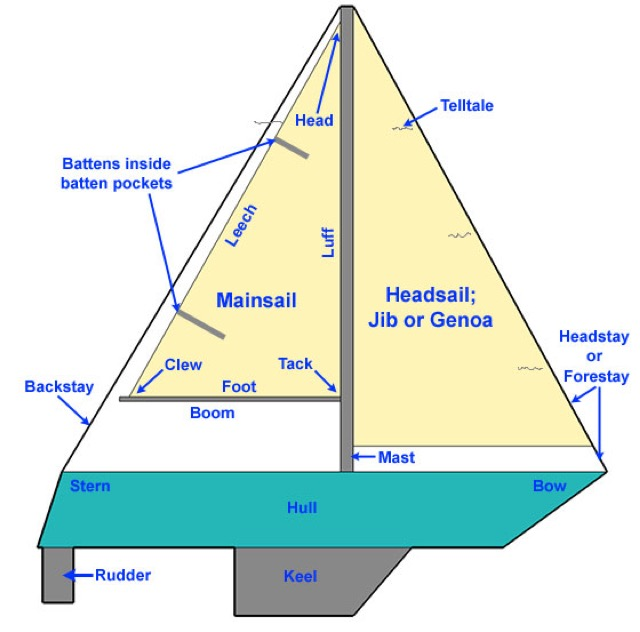
\includegraphics[width=0.4\linewidth]{sailboat_terms.jpg}
 \caption{Common sailboat terms \cite{sailboat_terms}. }
\label{sailboat_terms}
\end{figure}
\nomenclature[S]{$\lambda$}{Leeway Angle}
In order to steer a boat, the seamanship has to control the angle of the rudder, this interacts directly with the current, the direction obtained is called \textit{heading} and these two, rudder and current, generate forces that influence the boat to \textit{yaw}. \par
Due to the wind direction, mainly, the boat slips sideways and this effect is known as \textit{leeway}. The difference in course comparing with the heading is expressed as \textit{leeway angle ($\lambda$)}. %, which can be see in the figure \ref{forces_m} \textit{C}.
The sails adjustment is known as trim; when the trim reduce the area of the sail then the seaman is \textit{reefing}, most of the time this term refers to when the size of the sails is changing.  Reefing under sail allows the seamanship to control the wind intensity. \par
\nomenclature[S]{$M_{R}$}{Righting Moment}
The wind over the sails generates a force and an angle called \textit{heel angle}; which can be seen in figure \ref{forces_m} \textit{B}, this decreases the driving force. Under those circumstances, a moment is generated and to neutralize it, the seamanship generates a \textit{righting moment} (\textit{ $M_{R}$}) by standing on the windward side of the boat to produce it\cite{philpott1993yacht}. 
As a result of these forces, the velocity could be optimal or not. \cite{larsonprinciples} relates the factors and forces proposed in\cite{philpott1993yacht} in terms of forces and resistances, indicating how the dynamics of each of the mediums, water, and air, interact to keep the balance (and be capable to maximize the boat's speed). Therefore, the forces and resistances are related as showed below: \par 
\begin{itemize}  \label{milgramforces}
 \setlength \itemsep{0em}
\item Aerodynamic driving forces = Hydrodynamic resistance;
\item Aerodynamic side force = Hydrodynamic side force;
\item Aerodynamic heeling moment=Hydrodynamic (static) righting moment.
\end{itemize}
An important assumption made by  \cite{philpott1993yacht} and \cite{larsonprinciples} to keep the analysis of the boat in 2 dimensions is that vertical forces are in balance always, same as the pitching moment; Figure \ref{forces_m} \textbf{c} shows the only forces that act when this assumption is made; additionally 2 angles are shown, one of then refers to the wind.\par
\nomenclature[A]{DOF}{Degrees of freedom}
\section{Planes of motion} \label{sec:planes_motio}
Sailing boats are considered rigid bodies that can move in a three-dimensional space; figure \ref{DOF} shows the 6 fundamental types of motion or degrees of freedom (DOF)  with the names and axis where they are referred: three translations and three rotations. \par 
It also shows the water surface which is represented by the plane \textit{XY} and the orientation of the sailboat shows the positive direction of the three axes which follow the right-hand orthogonal system. Thus, \textit{X-axis} is positive in the direction of the motion, \textit{Y} is positive to port or left side of the sailboat and \textit{Z} is positive upwards. In the case of the \textit{Y-axis}, the negative direction or right side of the sailboat is known as starboard.  Besides, for future references, the speed of the boat is along the \textit{X-axis}. These six DOF correspond to three forces and three moments which are going to explain in the next section. \par 
\begin{figure} %[ht]
\centering
  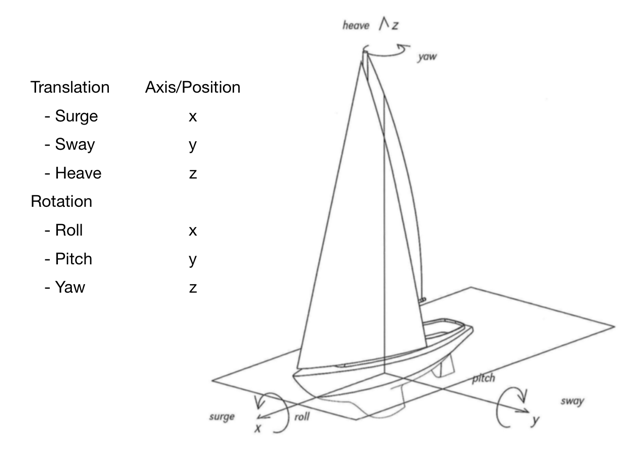
\includegraphics[width=0.7\linewidth]{dof_foss_modif.png}
 \caption{Degrees of freedom of a boat, clockwise reference system \textit{XYZ} \cite{fossati2009aero}. }
\label{DOF}
\end{figure}

%The information provided in the figure %To represent the position, velocities and forces, a set of vectors are defined in 

Because the sailboat interacts between two fluids not only do they generate forces but also resistances in both mediums. It is important to know how the elements are named and which words are related with a specific axis and  %These simple concepts are useful to understand how the equilibrium is generated in the static condition, 
which elements interact on it and how it is conserved when the sailboat moves from one point to another. \par 

\section{Hydrodynamic and Aerodynamic Forces and Momentum} \label{section:forces_moment}
The static and dynamic balance of any type of boat is based on Newton's second law. However, when the boat moves, a dynamic situation, it is the winds' velocity that leads to this equilibrium. Because the sailboat interacts between two fluids they not only generate forces but also resistances.
\nomenclature[S]{$F_{A}$}{Total Aerodynamic Force}
\nomenclature[S]{$F_{H_{TOT}}$}{Total Hydrodynamic Force}
The next equations basically show that the total aerodynamic force ($F_{A}$) is equal and opposite to the total hydrodynamic force ($F_{H_{TOT}}$). \par
From section \ref{sec:planes_motio}, a set of vectors can be defined to represent the position, velocities, and forces. The notation used here is similar to the one used by the \acrfull{sname} %\acrlong{sname} (\textit{\acrshort{sname}})%the Society of Naval Architects and Marine Engineers (\textit{SNAME}) 
because different authors use different notation, this work is intended to stay close to the norm which is shown in table \ref{table:SNAME_notation}, this notation refers to the body-fixed reference frame.
\nomenclature[A]{\textbf{SNAME}}{Society of Naval Architects and Marine Engineers}
\begin{table}%[]
    \centering
    \begin{tabular}{c|c|c|c}
    \hline
          Motion/Rotation & Force/Moment & Linear/Angular vel & Position/Angles   \\
    \hline 
         Surge(X-axis) & X & u & x \\  
         Sway (Y-axis) & Y & v & y \\
         Heave(Z-axis) & Z & w & z \\
         Roll (X-axis) & K & p & $\phi$ \\
         Pitch (Y-axis) & M & q & $\theta$\\
         Yaw (Z-axis) & N & r & $\psi$\\
    \end{tabular}
    \caption{\acrshort{sname}'s notation for motion components \cite{Alves2014ASailboat}}
    \label{table:SNAME_notation}
\end{table}

\nomenclature[S]{$\theta$}{Pitch Angle}
\nomenclature[S]{$\phi$}{Roll Angle}
\nomenclature[S]{$\psi$}{Yaw Angle}

\subsection{Wind and the Velocity Triangle} \label{sec:wind_vel_trian}
\nomenclature[S]{$V_{tw}$}{True Wind Velocity}
\nomenclature[S]{$\beta_{tw}$}{True Wind Angle}
\nomenclature[S]{$\kappa$}{Exponent for wind velocity at different height [1/7,1/4]}
In sailing, the wind is characterized by its speed and direction and it is defined as \textit{true wind velocity ($V_{tw}$)} and \textit{true wind angle ($\beta_{tw}$)}. Because it also interacts with the water surface, in some cases its intensity depends on the height where it was measured, to know its value at a different height it is estimated by equation \ref{eq:wind_h}. According to \cite{claughton1998sailing} the exponent $\kappa$ has a value between 1/7 and 1/14, and; the reference height for measurements is 10m above the water surface. \par 
\begin{equation}\label{eq:wind_h}
    V_{tw}(Z)=V_{tw}(Z_{ref}) \cdot \bigg( \frac{Z}{Z_{ref}} \bigg)^\kappa
\end{equation}

The steady motion of the sailboat not only depends on the balance of forces but also on the relation between velocities, boat, and wind, mainly. This interaction is represented by the velocity triangle shown in figure \ref{vel_triangle}. The triangle introduces the apparent wind velocity ($V_{aw}$) and angle ($\beta_{aw}$).\par 
\nomenclature[S]{$V_{aw}$}{Apparent Wind Velocity}
\nomenclature[S]{$\beta_{aw}$}{Apparent Wind Angle}
%\begin{figure}[ht]
%\centering
%  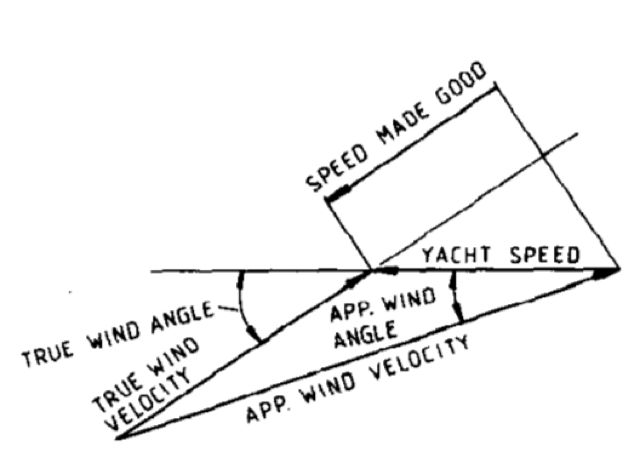
\includegraphics[width=0.65\linewidth]{Larsson_triang_vel.png}
% \caption{Velocity triangle  \cite{larsonprinciples}. }
%\label{vel_triangle_old}
%\end{figure}

%option figure to REVIEW
\begin{figure} %[ht]
  \centering
  \subfloat[Velocity triangle  \cite{larsonprinciples}. ]{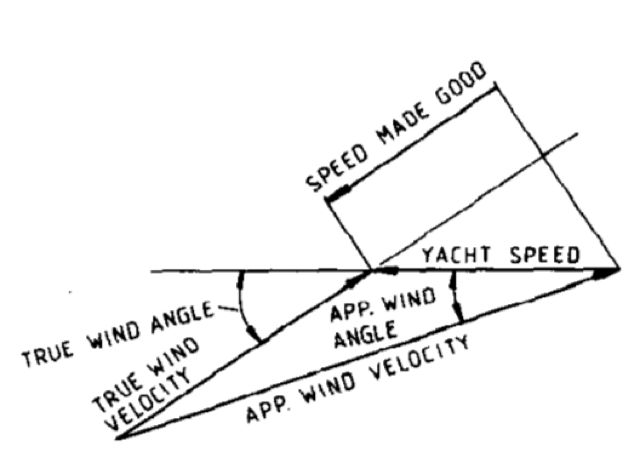
\includegraphics[width=0.45\linewidth]{Larsson_triang_vel.png}\label{vel_triangle}}
  \hfill
  \subfloat[Angles and course direction \cite{marchajaereo1979}.]{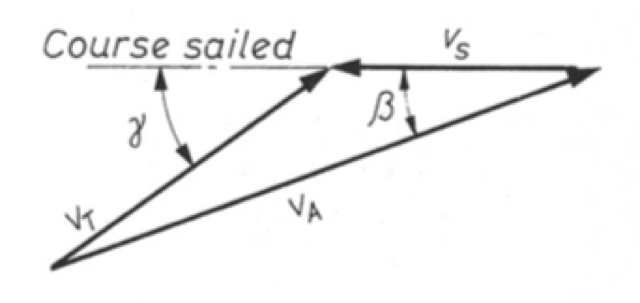
\includegraphics[width=0.45\hsize]{geo_vel_triangle}\label{fig:velTriang_sailCourse}}
  \caption{Velocity Triangle and angle directions of wind and $\lambda$  \cite{marchajaereo1979}, \cite{larsonprinciples}.}
\label{fig:Vel_Trian_Ang} 
\end{figure}

\nomenclature[S]{$V_{aw}$}{Apparent wind velocity}
%\nomenclature[A]{SGP}{Some Random Acronym}
%\newacronym{gcd}{GCD}{Greatest Common Divisor}
%EXAMPLE \acrlong{gcd} \acrfull{gcd} \acrshort{gcd} \acronymtype 

\nomenclature[S]{$\Theta$}{Heel Angle}
\nomenclature[S]{$\gamma$}{Course Angle}
\nomenclature[A]{$CE$}{Center of Effort}
\nomenclature[S]{$V_{boat}$}{Boat's velocity}

The $V_{aw}$ and $\beta_{aw}$ result from the vector summation of the true wind ($V_{tw}$) and sailboat's ($V_{boat}$) velocity, \ref{eq:vel_appVector}; a more complete estimation of them uses the heel angle ($\Theta$), equations \ref{eq:app_angle} and \ref{eq:app_angle} show how to calculate them. These equations include the heel angle because $V_{aw}$ is used to calculate some sail force coefficients which are specified at the center of effort (\textit{CE}), its location is about 40\% at the mast height. The $\beta_{aw}$ incorporated the leeway angle ($\lambda$), which value is usually less than 6\degree \cite{philpott1993yacht},\cite{claughton1998sailing}. Subsequently, the course angle $\gamma$ is complementary to the $\beta_{aw}$ when $\lambda$ is not bigger than 6\degree \ref{fig:velTriang_sailCourse}. \par
\begin{equation}\label{eq:vel_appVector}
    \vv{V_{aw}}=\vv{V_{tw}}-\vv{V_{boat}}
\end{equation}

\begin{equation} \label{eq:app_angle}
    \beta_{aw}=tan^{-1} \bigg( \frac{ V_{tw} sin \beta_{tw} cos \Theta }{ V_{tw} cos \beta_{tw} + V_{boat}} \bigg)
\end{equation}
\newline
\begin{equation} \label{eq:ap_vel}
    V_{aw}=  \sqrt{ (V_{tw} sin \beta_{tw} cos \Theta)^2 + (V_{tw} cos \beta_{tw} + V_{boat})^2}
\end{equation}

\subsection {Equilibrium Equations} \label{sec:equil_equat}
In the static condition, equilibrium is reached when the summation of all the forces and momentum equals zero. In figure \ref{forces_m} these forces are located according to the planes where they act, the names of them and the fluid that drives them. In addition to the forces and momentum, there are 4 angles to consider. Another observation is how the position and weight of the athlete are incorporated in the equilibrium equations. \par 

\nomenclature[A]{$\textit{F}$}{Force}
\nomenclature[S]{$F_{R}$}{Driving Force}
\nomenclature[S]{$R$}{Water Resistance}
\nomenclature[S]{$F_{H}$}{Heeling Force}

The equations of forces(\textit{F}) by plane in equilibrium are:
\begin{equation}\label{eq:force_x}
    \text{(Surge, x  \space axis)  \space} F_{R}=R \\
\end{equation}
\begin{equation}\label{eq:force_y}
    \text{(Sway, y\space axis) \space } \space F_{H,lat}=F_{S,lat}\\
\end{equation}
\begin{equation}\label{eq:force_z}
    \text{(Heave, z\space axis)  } \space F_{V}=F_{VW}
\end{equation}
And those for the momentum (\textit{M}) in equilibrium are:
\begin{equation}\label{eq:m_x}
    \text{(Roll, x  \space axis) \space } M_{R}=M_{H} \\
\end{equation}
\begin{equation}\label{eq:m_y}
    \text{(Pitch, y \space axis)  } \space M_{PA}=F_{PW}\\
\end{equation}
\begin{equation}\label{eq:m_z}
    \text{(Yaw, z \space axis)  } \space M_{YW}=M_{YL}
\end{equation}

 \begin{figure}[ht]
\centering
  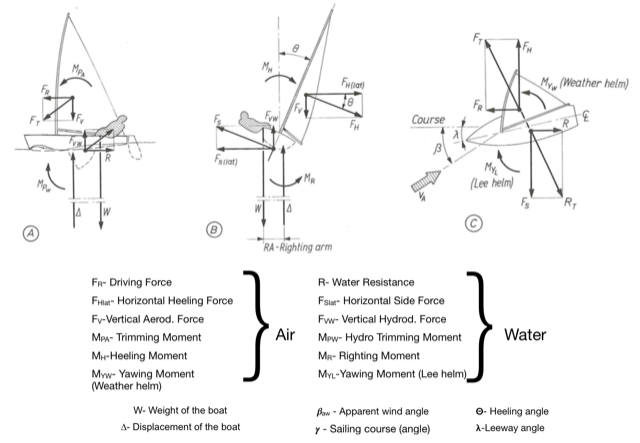
\includegraphics[width=.97\linewidth]{marchaj_forcesM.png}
 \caption{Equilibrium of forces and moments in steady-state sailing condition \cite{marchajaereo1979} }
\label{forces_m}
\end{figure}

\subsection{Aerodynamic Forces and Resistances} \label{sec:aero_forces}
\nomenclature[S]{$F_{S}$}{Hydrodynamic Side Force}
\nomenclature[S]{D}{Drag Force}
\nomenclature[S]{L}{Lift Force}

The force that drives motion of the sailboat is the driving force($F_{R}$); figure \ref{forces_m} \textit{B} shows the force that causes the drift (heel) of the sailboat is the heeling force ($F_{H}$). The motion of the sailboat happens when $F_{R}$ beat the hull resistance (\textit{R}); while in the \textit{ZY} plane the balance of the forces happens when $F_{H}$ equals the hydrodynamic side force ($F_{S}$), which is produced by the effect of the water over the hull. Then:\par 
\begin{figure} [htb!]
    \centering
    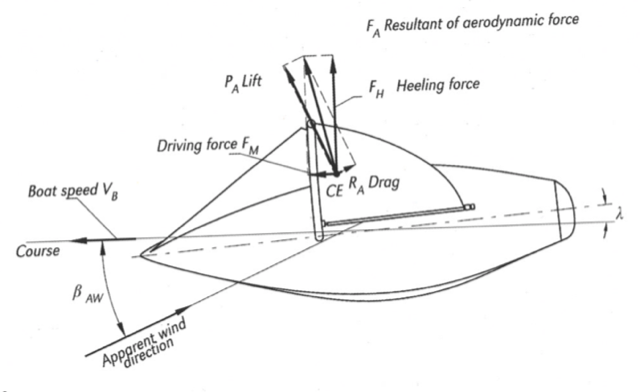
\includegraphics[width=.5\linewidth]{Ftot_aereo.png}
    \caption{Total Aerodynamic Forces \cite{fossati2009aero}}
    \label{fig:Ftot_aereo}
\end{figure}
%( Because $F_{A}$ result from $F_{R}$, parallel to the \textit{apparent wind} direction and $F_{H}$ perpendicular to $F_{R}$. Under balance the variables related to them are:)
\begin{multline}
\\
F_{A}=F_{R}(\parallel V_{aw}) + F_{H}(\bot F_{R} )\\
F_{R}=F_{R}(V_{aw},\beta_{aw}, \Theta) \\
F_{H}=F_{R}(V_{aw},\beta_{aw}, \Theta) \\
F_{S_{lat}}=F_{S}(V_{boat},\lambda, \Theta) \\
R=R(V_{boat},\lambda, \Theta)\\  
\end{multline}
%th they depend on the $V_{aw}$ and $\beta_{a}$; while $F_{S}$ and \textit{R} depend on $V_{boat}$ and $\lambda$. 
Due to the dependency on velocities, $F_{R}$ and $F_{H}$ generate drag (\textit{D}) and lift (\textit{L}) forces acting normal to the center plane of the hull and mast and they are integrated into the forces, figure \ref{fig:Ftot_aereo}, according to \cite{philpott1993yacht} and \cite{claughton1998sailing} as: \par 
\begin{equation} \label{eq:Fr_LD}
    F_{R}=L sin \beta_{a} - D cos \beta_{a}
\end{equation}
\begin{equation} \label{eq:Fh_LD}
    F_{H}=(L cos \beta_{aw} + D sin \beta_{aw}) cos\Theta
\end{equation}
\\ \textit{D} and \textit{L} depends not only on  the sail area (\textit{$A_{s}$)}, $V_{aw}$, and fluid density ($\rho_{a}$), in this case, air, but also on coefficients which depends on the trim and flatness of the sail \cite{philpott1993yacht}, \cite{carrico17symp}, \cite{day2017performance}; these last, are under the control of the seamanship. \textit{D} and \textit{L}  are expressed in those terms as follow: \par
\nomenclature[S]{$\rho_{a}$}{Air Density}
\begin{equation} \label{eq:Lift}
  L=qA_{s}C_{t}  
\end{equation}
\begin{equation} \label{eq:Draf}
    D=qA_{s}C_{d}  
\end{equation}
\begin{equation} \label{eq:dynamic_press}
    q=\frac{1}{2}\rho_{a} V_{aw}^2
\end{equation}
\begin{equation} \label{eq:Cd}
    C_{d}=C_{d}(\beta_{a},trim, flatness)
\end{equation}
\begin{equation} \label{eq:Ct}
    C_{t}=C_{t}(\beta_{a},trim, flatness)
\end{equation}
where:
\begin{itemize} \label{ae_symbols}
    \item $\rho_{a}$ air density approx. 1.225 $kg/m^3$.
    \item $A_{s}$ is the area of the sail.
\end{itemize}

\nomenclature[S]{$A_{s}$}{Sail Area}
\nomenclature[S]{$F_{ms}$}{Driven Sail Force}
\nomenclature[S]{$F_{ss}$}{Side Sail Force}
\nomenclature[S]{$q$}{Dynamic Pressure}

$C_{d}$ and $C_{t}$ values are obtained from tables or graphics and their range is over (0,1), later on, this is going to be explained in detail. \par 
$F_{R}$ is the total force applied on the sail which can be decomposed in 2 more forces; a driven force $F_{ms}$ and a side force $F_{ss}$ expressed in the terms mentioned before as:\par
\begin{equation}\label{eq:drive_sail_force}
    F_{ms}= (L cos \beta_{aw}+ D sin \beta_{aw})cos \Theta sin \lambda + (L sin \beta_{aw}-D cos\beta_{aw})cos \lambda
\end{equation}
\begin{equation}\label{eq:side_sail_force}
    F_{ss}=(L cos \beta_{aw}+ D sin \beta_{aw})cos \Theta cos \lambda - (L sin \beta_{aw}-D cos\beta_{aw})sin \lambda
\end{equation}
%%%NEW SUBSECTION %%%
\subsection {Hydrodynamic Forces and Resistances} \label{sec:hydroforces}
$F_{H_{TOT}}$ is equivalent to $F_{A}$ with the difference that they result from the interaction with the water. In this case, \textit{R}, a drag force (resistance) oppose the motion of the sailboat as shown in figure \ref{fig:Ftot_hydro}; and the horizontal side force $F_{S_{lat}}$, is a lift force acting over the hull and keel. Most of the information related with the modeling of the hull and keel is based on experimental data. % which is used to calibrate the theoretical model.
Then the drag generated by the hull is the result of the  upright, heeled and induced resistances \cite{philpott1993yacht}.\par

\nomenclature[S]{$F_{S_{lat}}$}{Horizontal Side Force}
\nomenclature[S]{$C_{d}$}{Drag Coefficient}
\nomenclature[S]{$C_{t}$}{Lift Coefficient}

\begin{equation}
    F_{H_{TOT}}=R(\parallel( -V_{aw})) + F_{S_{lat}}(\bot R )\\
\end{equation}

\begin{figure}
    \centering
    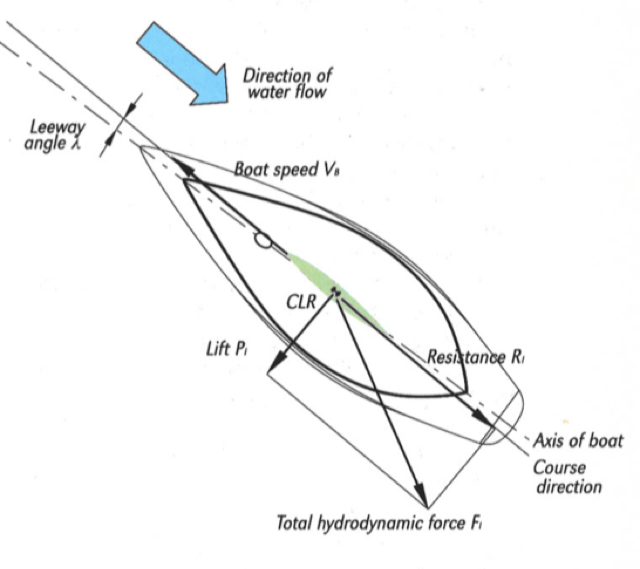
\includegraphics[width=.5\linewidth]{Ftot_hydro.png}
    \caption{Total Hydrodynamic forces. \cite{fossati2009aero}}
    \label{fig:Ftot_hydro}
\end{figure}

The upright resistance is produced by the hull drag and when $\lambda$ is zero. It is constituted by the friction generated by the water viscosity and wave drag, dissipation of energy in form of waves due to the shape of the hull. The formula to calculate these two frictional forces, equation \ref{eq:water_fric} and \ref{eq:wave_fric} is similar to the one from classical hydrodynamics, the difference is the coefficients. $C_{f}$ depends on $V_{boat}$ and its waterline length while $C_{w}$ depends on the hull shape and Froude number (\textit{Fr}), which considers the $V_{boat}$ and length of the sailboat; however, it is often determined by tests evaluations.
\nomenclature[S]{$C_{f}$}{Hydrodynamic Coefficient for the waterline length}
\nomenclature[S]{$C_{w}$}{Hydrodynamic Coefficient for the hull shape}
\nomenclature[S]{$F_{i}$}{Induced and heeled resistance forces}

\begin{equation}\label{eq:water_fric}
 F_{f}=\frac{1}{2}\rho_{w} C_{f} A_{w} V_{boat}^2
\end{equation}
\begin{equation}\label{eq:wave_fric}
 F_{w}=\frac{1}{2}\rho_{w} C_{w} A_{w} V_{boat}^2
\end{equation}
where:
\begin{itemize} \label{R_symbols}
    \item $\rho_{w}$ water density approx. 1000 $kg/m^3$.
    \item $A_{w}$ is the wetted surface area of the sailboat
\end{itemize}
\nomenclature[S]{$A_{w}$}{Wetted Surface Area of the sailboat}
\nomenclature[S]{$\rho_{w}$}{Water Density}

The induced and heeled resistances are combined and related with the heel and $\lambda$, its formula also depends on $V_{boat}$. Due to its complex derivation and different versions the expression is going to be set as; $F_{i}(\lambda,\Theta,V_{boat})$, for the purpose of this work. Then \textit{R} due to hydraulic resistances is calculated as: \par 
\begin{equation} \label{eq:R_total}
    R=F_{f}+F_{w}+F_{i}
\end{equation}

\nomenclature[S]{$S$}{Total Side Force}

In the case of $F_{S_{lat}}$, it depends also on 3 resistances generated by the hull, the lifting surface of the rudder and keel; these 2 last are the more significant and they are also perpendicular to the velocity. This total side force (\textit{S}), on the water plane, depends on the plan area of the keel and rudder and in 2 coefficients, respectively.  Thus, it is estimated as: \par 

\begin{equation} \label{eq:Side_force}
    S=\frac{1}{2} \rho_{w} V_{boat}^2(C_{rudder}A_{rudder}+C_{keel}A_{keel})cos \Theta
\end{equation}.

\nomenclature[S]{$C_{rudder}$}{Rudder Coefficient}
\nomenclature[S]{$C_{keel}$}{Keel Coefficient}
\nomenclature[S]{$A_{rudder}$}{Rudder Surface Area}
\nomenclature[S]{$A_{keel}$}{Keel Surface Area}

The shape, of the rudder and keel, in conjunction with the angle of attack, has implication on each coefficients respectively. %$C_{rudder}$ and $C_{keel}$, each depends on the the shape and angle of attack of each. 
The angle of the rudder ($\beta_{r}$) is the angle it makes with the center line of the sailboat. Each angle of attack (\textit{$\beta_{i_{a}}$})is determined as: \par 
\nomenclature[S]{$\beta_{r}$}{Rudder Angle}
\nomenclature[S]{$\beta_{r_{a}}$}{Rudder Angle of Attack}
\nomenclature[S]{$\beta_{k_{a}}$}{Keel Angle of Attack}
\begin{equation} \label{eq:att_r}
    \beta_{r_{a}}=tan ^{-1} (cos \Theta cos \lambda + \beta_{r})
\end{equation}
\begin{equation}  \label{eq:att_k}
    \beta_{k_{a}}=tan ^{-1} (cos \Theta cos \lambda )
\end{equation}

$F_{S_{lat}}$ in equilibrium can be estimated based by using $F_{H}$ which generates a reaction force below the water surface, then: %
which us know as horizontal side force $F_{S_{lat}}$ and it is determined as follow: \par
\begin{equation}
    F_{Slat}= F_{H}cos \Theta
\end{equation}

%% new section
\nomenclature[A]{$CLR$}{Center of Lateral Resistance}
\nomenclature[S]{$M_{R}$}{Righting Moment}
\nomenclature[S]{$W$}{Weight}

\subsection{Momentum at the sailboat model} \label{sec:momentum_types}
Because $F_{A}$ is applied at \textit{CE}, above the waterline and located over the sails area; and $F_{H_Tot}$ at the center of lateral resistance (\textit{CLR}), defined below the waterline. The moments generated over the sailboat depends on these 4 variables. For example, the \textit{righting moment ($M_{R}$)}, figure \ref{forces_m} \textit{B} is counterbalanced as next: 
\begin{equation}\label{eq:right_mom}
    M_{R}=F_{H}(CE-CLR)_{z}=W \cdot RA
\end{equation}
where:\par
\begin{itemize}
    \item $(CE-CLR)_{z}$ is the heeling arm or the vertical distance between \textit{CE} and \textit{CLR} when $F_{H}$ is perpendicular to it.
    \item W = weight of the boat.
    \item RA = Righting arm or the horizontal distance between the \textit{W} and the \textit{Z} axis.
\end{itemize}
\nomenclature[S]{RA}{Righting Arm}
\nomenclature[S]{$W_{c}$}{Weight of the crew}
This expression does not take into account the weight of the crew. The moment generated by the crew weight is given by the weight of the crew (\textit{$W_{c}$})) and its relative position to the centerline of the boat, which is expressed by a variable known as \textit{$y_{c}$}. This variable has a range value of [-1,1], and if the crew is in the centerline then its value is zero. Another factor to considers is $\Theta$. So the moment generated by the crew according to Philpott \cite{philpott1993yacht} is: \par 
 \nomenclature[S]{$y_{c}$}{Crew position on Y-axis from the centerline}
 \nomenclature[S]{$M_{c}$}{Crew Moment}
 
\begin{equation}\label{eq:Moment_crew}
    M_{c} = y_{c} W_{c} Y_{max} cos \Theta
\end{equation} 
\begin{equation} \label{eq:Mcrew_dist}
    Y_{max} = \frac{1}{2} beam(width)_{sailboat}
\end{equation}

\nomenclature[S]{$M_{R_{TOT}}$}{Total Righting Moment}

and the \textit{total righting moment ($M_{R_{TOT}}$)} is:
\begin{equation} \label{eq:Mr_tot}
    M_{R_{TOT}}=M_{R}(V_{boat}, \Theta, \lambda) + M_{c}
\end{equation}

\nomenclature[S]{$M_{Y}$}{Yaw Moment}
\nomenclature[S]{$R_{hull}$}{Hull Resistance}
The \textit{yaw moment} $(M_{Y})$ causes the rotation on the \textit{Z-axis} and depends on the rudder angle (\textit{$\beta_{r}$}), most of the time, since it can shift the \textit{CLR}, another way to change this distance is by trimming, which changes the area of the sail, therefore, the \textit{CE} shifts its location. If the sailing motion is steady then this moment is zero; otherwise, it can be calculated by the hydrodynamic resistance from the hull and the from the keel and rudder side forces; which are compensated by the sail forces \cite{philpott1993yacht}, \cite{claughton1998sailing}. These 3 forces generated the $(M_{Y})$, as shown next: \par
\begin{equation}\label{eq:Hull_R}
    R_{hull}=R+F_{H}=F_{f}+F_{w}+F_{H}
\end{equation}
\begin{equation}\label{eq:hull_moment}
   M_{hull}=R_{hull}(CLR_{y} cos \lambda sin \Theta - x_{y} sin \lambda cos \Theta) 
\end{equation}
\begin{equation}\label{eq:keel-rudder_moment}
   M_{k-r}=\frac{1}{2}\rho_{w} V_{boat}^2(C_{rudder}A_{rudder}x_{r}+C_{keel}A_{keel}x_{k})cos \Theta cos \lambda
\end{equation}
\begin{equation}\label{eq:sail_moment}
    M_{sail}=x_{s}F_{ss}+z_{0}r sin \Theta F_{ms}) cos \lambda
\end{equation}

\nomenclature[S]{$x_{y}$}{Distance of the CLR from the \textit{Z-axis}}
\nomenclature[S]{$x_{r}$}{Lever Arm of the Rudder}
\nomenclature[S]{$x_{k}$}{Lever Arm of the Keel}
\nomenclature[S]{$x_{s}$}{CE distance from the yaw axis (Z-axis)}
\nomenclature[S]{$z_{0}r$}{Lever Arm of the CE}
\nomenclature[S]{$r$}{Reefed/trim proportion of the sail}
\nomenclature[S]{$z_{0}$}{Height of the CE}
\nomenclature[S]{$M_{sail}$}{Total Sail Moment}
\nomenclature[S]{$M_{hull}$}{Hull Moment}
\nomenclature[S]{$M_{k-r}$}{Moment produced by the keel and rudder}

The \ref{eq:hull_moment} uses $x_{y}$ which refers to the distance of the \textit{CLR} from the \textit{Z-axis} (\textit{yaw axis}) while in \ref{eq:keel-rudder_moment} $x_{r}$ and $x_{k}$ are the lever arms of the rudder and keel, respectively, finally in \ref{eq:sail_moment} $x_{s}$ is the distance from the yaw axis to the \textit{CE} and $z_{0}r$ is the lever arm of it, where $z_{0}$ is the height of the \textit{CE}  and \textit{r} is the reefed/trim proportion of the sail. As mentioned in section \ref{sec:wind_vel_trian} $\lambda$ is small which allows cos and sin functions to be simplified by linear approximations. \par 

\nomenclature[S]{$M_{P}$}{Trimming Moment}
\nomenclature[A]{$g$}{gravity}
\nomenclature[S]{$\Delta$}{Vertical Displacement of the boat, related with the buoyancy when the boat is static}

The \textit{trimming moment} ($M_{P}$) arise from gravity (\textit{g}) and buoyancy forces, the displacement of the boat (\textit{$\Delta$}) is related with $V_{boat}$ ; for example, at high velocities, the lift forces are added to the buoyancy forces at the front sections. 

In case of rough water, however, the pitching motion reduces the speed and it is compensated by the aerodynamic and hydrodynamic forces\cite{claughton1998sailing}.\par 

The equilibrium of forces and moments of the sailboat results from the interaction between the forces generated by the air, or by  water or by both into different parts of the sailboat. These interactions in some cases are sophisticated. One of the reasons is the values that depend on coefficients related with the shape of the particular element of the sailboat and the condition of the wind beside the fact that the density value of each medium is different. The steady motion is reached when all these forces are in equilibrium considering the wind and its direction. Due to the complexity of the relation above the solution or equilibrium condition is not unique. Because of these, it is possible to sail at different directions and to reach a place even when it is on on the windward side of the sailboat. 
%%% NEW SECTION%%%%%
\section{Velocity Prediction Polar} \label{sec:VPP}

\nomenclature[A]{$VPP$}{Velocity Prediction Program/Polar}

In 1979 scientists developed the velocity prediction  program (\textit{VPP}) with the objective to predict the sailboat speed and direction for any wind condition, magnitude, and direction \cite{larsonprinciples}. The results can be interpreted easily using a polar diagram or by reading its results in the form of tables.  The kinetics of the sailboat explains how the motive forces from sails equal the hull resistance and how side forces from keel and rudder equal the sail side forces; in other words, how the aerodynamic forces and momentum are counterbalanced by the hydrodynamics of it. These relations and results are obtained from the static equilibrium equations mentioned in section \ref{sec:equil_equat}.\par 
\begin{figure}
    \centering
    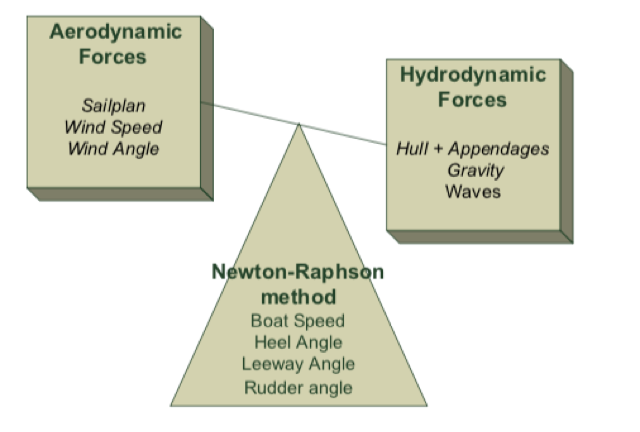
\includegraphics[width=0.5\hsize]{images/Vpp_balance_eq.png}
    \caption{VPP Force Balance Representation \cite{bohm2014velocity} }
    \label{fig:my_label}
\end{figure}
The VPP contains the solutions of the equations to accomplish this balance and it requires not only to solve the hydrodynamic and aerodynamic equations but also to know the properties of the sailboat related with its stability, such as $\lambda$ \cite{larsonprinciples}, \cite{milgram1998fluid}. The information required to get a VPP comes from different sources and all the variables involved can be classified in 4 categories or groups, according to \cite{philpott1993yacht} these groups are:
\begin{itemize}
    \item design (\textit{$_{d}$}): describe the size and shape of the sailboat and its elements.
    \item environment (\textit{$_{e}$}): describe the wind and current in which the sailboat will perform.
    \item control (\textit{$_{x_{c}}$}): these are setting variables that can be adjusted within some limits or constraints by the seamanship, such as $\beta_{r}$, $y_{c}$, \textit{f}, and \textit{r}.
    \item behavior (\textit{$_{y_{b}}$}): these variables describe the motion or condition of the motion at a given time or due to a given environmental condition. Examples of this type or variables are: $\lambda$, $\beta_{tw}$, $\Theta$, and the $V_{boat}$
\end{itemize}

\nomenclature[S]{$_{d}$}{Subscript for Design Variables}
\nomenclature[S]{$_{e}$}{Subscript for Environment Variables}
\nomenclature[S]{$x_{c}$}{Subscript for Control Variables}
\nomenclature[S]{$y_{b}$}{Subscript for Behavior Variables}
\nomenclature[S]{${aux}$}{Subscript for Auxiliary Variables}

The rest of the variables can be grouped as \textit{auxiliary} variables (\textit{$_{aux}$}). These variables describe transitional stages or intermediate calculations, such as $V_{aw}$, \textit{D}, \textit{L}, $M_{c}$, $M_{sail}$ among others. The arrangement of these groups results in at least 22 simultaneous nonlinear equations which can be solved by specifying a performance criterion and optimizing the \textit{$_{y_{b}}$} variables.
%From the equations of previous sections 18 variables were identiy as \textit{aux}.  
 
Because VPP plots are symmetric only half of it is usually represented as shown in figure \ref {typ_vpp}. The polar diagram indicates the wind direction or \textit{true wind angle} at 0\degree , $V_{boat}$ is defined by the radius size of the concentric half circles, the straight lines indicate the direction of the boat from the wind direction. Last, the wind speed is the group of lines that form a half heart shape; the intersection of these lines with direction lines indicates the maximum velocity that a sailboat can attain. \par 
\begin{figure} %[ht]
  \centering
  \subfloat[VPP plot for true wind angles from 0 \degree to 180\degree and true wind speeds from 4 to 10 m/s (7.77-19.44 kn) \cite{larsonprinciples}.]{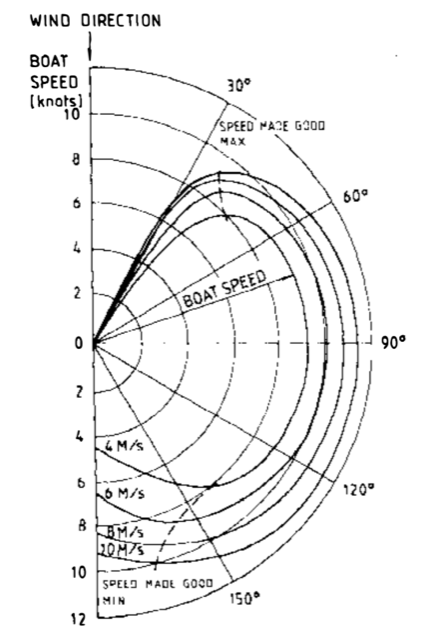
\includegraphics[width=0.38\linewidth]{vppLarsson1990.png}\label{typ_vpp}}
  \hfill
  \subfloat[Polar Curve of the Propulsion System \cite{yang2011control}(Full VPP representation).]{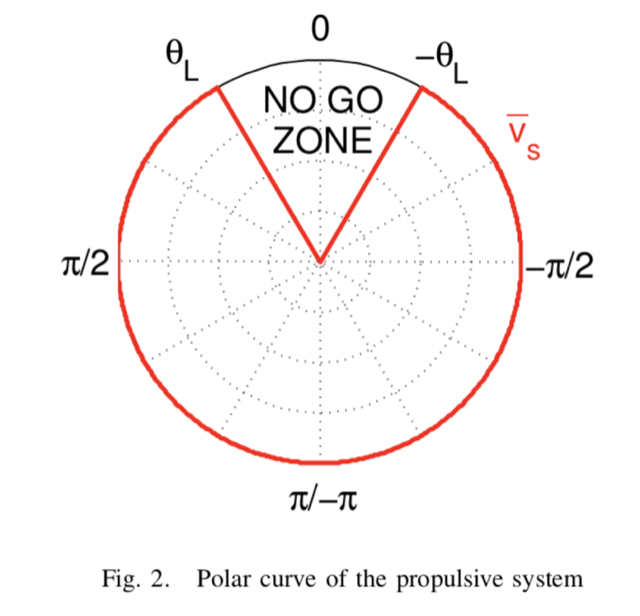
\includegraphics[width=0.45\hsize]{no-go_zone_yang.png}\label{no_go_zone}}
  \caption{VPP diagram}
\label{vpp_diag} 
\end{figure}

By using the VPP not only the direction of the maximum sailboat speed can be identified but also it shows the direction where the speed is the slowest. The angle range of this speed or speeds corresponds to the concave curve of the true wind, the area is defined as the \textit{no-go-zone} and it represents the set of directions that should be avoided to stay away from the irons \cite{yang2011control},\cite{denny2009float}, which means that under these directions the sailboat  motion is minimal, its propulsion is no enough or minimal to outweigh the resistance derived from the hull and sail.\par 

The performance criterion most used is to maximize $V_{boat}$ except when the sailing is towards the wind, upwind condition or sailing to windward. In this case, the performance criterion change from velocity to the distance that can be travel during a certain time.  This criterion is known as the velocity made good \textit{(VMG)} and it indicates where the sailboat is on the space from a reference and how is its motion \cite{larsonprinciples}, \cite{marchajaereo1979} \cite{philpott1993yacht}. \par 
\noindent
\textit{VMG} is determined by equation \ref{eq:VMG}. This relation can also be found in the velocity triangle, figure \ref{vel_triangle}, a more detailed geometrical is the figure \ref{fig:vmg_marchal_book}, where it is possible to identify how the $\beta_{tw}$ and $\lambda$ interact to gets the $\beta_{aw}$ therefore, how distance from the origin or reference point can be optimized and how different angles perform with the same given time. \par
\nomenclature[A]{$VMG$}{Velocity Made Good}

\begin{equation}\label{eq:VMG}
\begin{aligned}
VMG &=  \mid V_{boat} cos \beta_{tw} \mid 
\end{aligned}
\end {equation}

\begin{figure}
    \centering
    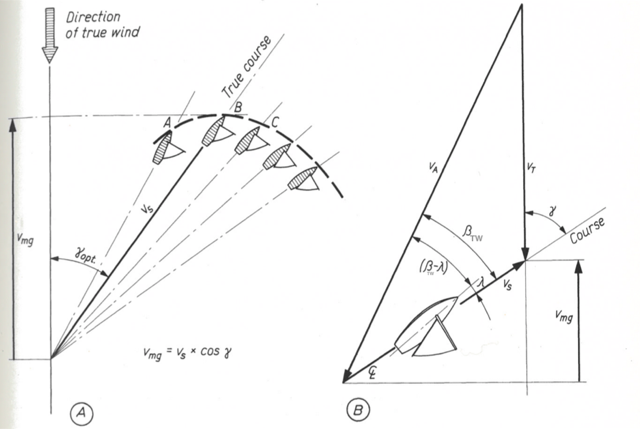
\includegraphics[width=0.75\linewidth]{vmg_marcha.png}
    \caption{Definition of VMG. A. VMG at  different angles. B. Velocity triangle including the leeway angle \cite{marchajaereo1979}.}
    \label{fig:vmg_marchal_book}
\end{figure}

The VPP is obtained by balancing the equations from previous sections, from equation \ref{eq:force_x} to equation \ref{eq:sail_moment}. It derives the $V_{boat}$ at different wind conditions and at different directions, angles respect to the wind. 

However, these equations are not usually solved in its six DOF. Because it was assumed that the vertical forces and moments are always in equilibrium, as was mentioned by \cite{larsonprinciples}, \cite{fossati2009aero} and on section \ref{sec:interaction_boat_environ}. The VPP partially solves the equations which means that the result provided only applies on 2D; particularly in the plane \textit{XY}. So it only considers the rolling moment and longitudinal forces  because changes on the \textit{Z} plane are neglected; but some of the variables related with the \textit{Z-axis} are considered, like $\Theta$. \par 
In this section, it was identified how the variables are categorized, most importantly which variables can be adjusted by the seamanship and which are defined by the sailboat and weather.


\section{Equations of Motion} \label{sec:eq_of_motion}
The motion of the boat from one point to another occurs in the XY plane. In the previous sections, the different components like forces generated by the wind and water were explained and how the seamanship or athlete compensate these forces by interacting with sailboat via sails,$\beta_{tw}$, and rudder, $\lambda$, mainly. On section \ref{section:forces_moment} 
it was mentioned that pitching moment and sway forces (vertical forces) are always in equilibrium, which means that heave and  pitch  motion can be omitted and the motion analysis only occurs on the XY plane within 4 DOF. These motions are the surge, sway, yaw, and roll.\par 

In 2004, de Keuning. et. al \cite{keuning2004mathematical} propose a mathematical model to describe the motion of sailboats or \textit{tacking maneuvers} with wide used parameters, like the information provided by the \textit{Delft Systematic Yacht Hull Series} (\textit{DSYHS}), so the estimation of the coefficients can be defined from this model without the need for experimental data for specific sailboat. \par 

\nomenclature[A]{$DSYHS$}{Delft Systematic Yacht Hull Series}

In the model, the main change refers to its coordinate system, figure \ref{fig:csys_tackmodel} shows the that the coordinate system is at the center of the sailboat, the \textit{Z-axis} is positive orientation when it points downwards and the \textit{Y-axis} is pointing at starboard \cite{keuning2004mathematical}. \par

\begin{figure} %[ht]
  \centering
  \subfloat[Motion depict by the mathematical model.]{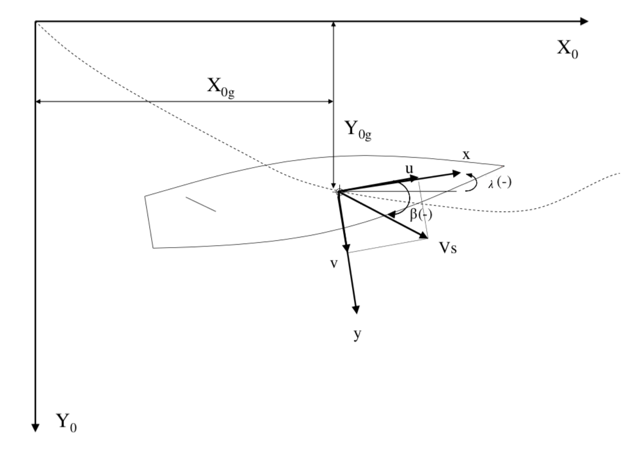
\includegraphics[width=0.38\linewidth]{ridder_motion.png}\label{fig:motion_csys_tackmodel}}
  \hfill
  \subfloat[Angle's location and axis orientation according to the coordinate system.]{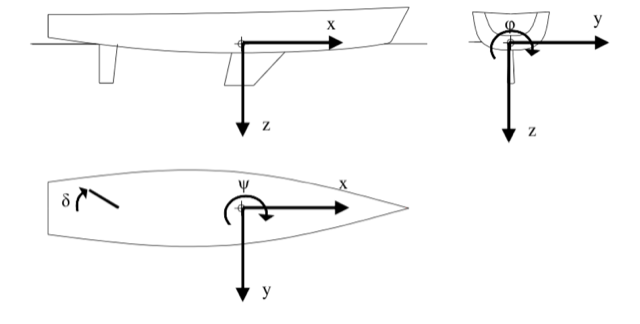
\includegraphics[width=0.45\hsize]{ridder_caxis.png}\label{fig:axis_cystackmodel}}
  \caption{Motion depiction of the mathematical model bestow by the coordinate system \cite{keuning2004mathematical}.}
\label{fig:csys_tackmodel} 
\end{figure}

The next equations or Euler's equations for sailboats motion described by \cite{keuning2004mathematical} define the total forces applied in the sailboat element corresponded to the main axis.\par

\nomenclature[S]{$X_{U}$}{Hull resistance in the upright position on the X direction}
\nomenclature[S]{$X_{i}$}{Forces in X direction of the \textit{i} element}
\nomenclature[S]{$Y_{i}$}{Forces in Y direction of the \textit{i} element}
\nomenclature[S]{u}{Velocity along the X direction}
\nomenclature[S]{v}{Velocity along the Y direction}
\nomenclature[S]{$\Dot{u}$}{Acceleration in the X direction}
\nomenclature[S]{$\Dot{v}$}{Acceleration in the Y direction}

The forces on the X and Y axis are: \\  
\begin{equation}\label{eq:force_X_motion}
    X_{U}+X_{hull}+X_{rudder}+X_{sail}=m_{T}(\Dot{u}-v\Dot{\psi})
\end{equation}
\begin{equation}\label{eq:force_Y_motion}
    Y_{hull}+X_{rudder}+X_{sail}=m_{T}(\Dot{v}-u\Dot{\psi})
\end{equation}
And the momentum on the X and Y axis are: \\
\begin{equation}\label{eq:moment_X_motion}
    K_{hull}+K_{rudder}+K_{sail}+K_{stability}=I_{xx} \Ddot{\phi}
\end{equation}
\begin{equation}\label{eq:moment_Y_motion}
    N_{hull}+N_{rudder}+N_{sail}=I_{zz} \Ddot{\psi}
\end{equation}
%<vertical forces are in balance always same as the pitching moment
where: 
\begin{itemize}  \label{symbols o motions}
 \setlength \itemsep{0em}
\item $m_{T}$ = the total mass of the sailboat not including crew.
\item u = velocity along the X-axis.
\item v= velocity along the Y-axis.
\item $\phi$ = roll angle, related to $\Theta$.
\item $\psi$ = yaw angle. %which is the course angle respect to the wind).
\item $I_{xx}$ = total mass moment of inertia in the roll axis (X.axis).
\item $I_{zz}$ = total mass moment of inertia in yaw axis (Z-axis).
\item K = Rolling moment (X-axis).
\item N = Yawing moment (Z-axis).
\item $X_{U}$ = is the hull resistance in the upright position.
%\item $X/Y_{hull}$ = is the resistance of the hull under the heeled resistance.
\end{itemize}

\nomenclature[S]{$m$}{Total mass of the sailboat including crew mass}
\nomenclature[S]{$K_{i}$}{Rolling moment (X-axis) of the \textit{i} element}
\nomenclature[S]{$N_{i}$}{Yawing moment (Y-axis) of the \textit{i} element}
\nomenclature[S]{$I_{ii}$}{Total mass moment of inertia in the \textit{i-axis}}

It is important to clarify that $\psi$ and $\phi$ are variables that describe the location of the sailboat over an area while and they are related with $\Theta$ and $\lambda$ from the kinematics of the sailboat; because the motion described by Keuning et. al \cite{keuning2004mathematical} includes waves effect because of this there is a difference between $\phi$ and $\Theta$. The heel angle $\Theta$ is the rotation from the \textit{Z} plane in \textit{flat water}; while $\phi$, the roll angle, is $\Theta$ plus the rotation induced by the fluctuations on the front wave \cite{kimball2009physics}, \cite{denny2009float}. \par 
\textit{ $ K_{stability} $ } is the moment generated by the weight when $\Theta$ is not zero; the center of buoyancy (\textit{B}) of the sailboat moves laterally and when its vertical line crosses the midplane of the sailboat creates a metacenter (\textit{M}). The distance between \textit{CG} and \textit{M} is known as the metacentric height, \textit{$\overline{GM}$} ) \cite{patterson2014ship} this displacement generates an oscillation and a mass moment that is calculated as follow:
\begin{equation} \label{eq:k_stability}
    K_{stability}=-mg\overline{GM} sin \phi 
\end{equation}

\nomenclature[A]{$B$}{Center of buoyancy}
\nomenclature[A]{$M$}{Metacenter}
\nomenclature[S]{$\overline{GM}$}{Metacentric Height}
\nomenclature[A]{$CG$}{Center of Gravity}

The rudder and the sail are sailboat elements controlled by the seamanship. 
The rudder produces hydrodynamic forces and momentum, as explained in section \ref{sec:momentum_types}; and the weight of the crew generates a momentum \ref{eq:Moment_crew} 
this momentum can be included on the previous equations by assuming that the centroid of $W_{c}$ is located in the center of gravity (\textit{CG}) and so forth the equations are:\par \noindent
Surge (X-axis):
\begin{multline}\label{eq:force_xMasuyama}
    X_{U}+X_{hull}+X_{rudder}+X_{sail}+X_{V\Dot{\psi}}V\Dot{\psi}\\ =(m+m_{x})\Dot{u}-(m+m_{y}cos^2\phi+m_{z}sin^2\phi)v\Dot{\psi}
\end{multline}
\\
Sway  (Y-axis):
\begin{multline}
\label{eq:force_yMasuyama}
Y_{hull} + Y_{rudder} + Y_{sail} + Y_{\Dot{\phi}} \Dot{\phi} + Y_{\Dot{\psi}} \Dot{\psi} \\ 
=\{(m + m_{y})cos^2 \phi + m_{z} sin^2 \phi \} \Dot{v} + (m + m_{x})u \Dot{\psi} + 2(m_{z} - m_{y}) sin\phi cos\phi \cdot v \Dot{\phi}
\end{multline}
\\
Roll (X-axis):
\begin{multline}
     K_{hull} + K_{rudder} + K_{sail} + K_{stability} +K_{\Dot{\phi}} \Dot{\phi} \\
 =(I_{xx} + J_{xx}) \Ddot{\phi} - {(I_{yy} + J_{yy})-(I_{zz} + J_{zz})} sin\phi cos\phi \cdot \Dot{\psi}^2
\end{multline}  \label{eq:m_xMasuyama}
\newline
Yaw (Z-axis):
\begin{multline}
   N_{hull}+N_{rudder}+N_{sail}+N_{\Dot{\psi}}\Dot{\psi}\\
 = \{ (I_{yy} + J_{yy}) sin^2 \phi +(I_{zz} + J_{zz})cos^2 \phi \} \Ddot{\psi} +2 \{(I_{yy} + J_{yy})-(I_{zz} + J_{zz})\}sin\phi cos\phi \cdot \Dot{\psi} \Dot{\phi}  
\end{multline}\label{eq:m_yMasuyama}
\newline
where: 
\begin{itemize}  \label{symbols_motions2}
 \setlength \itemsep{0em}
\item m = mass of the boat without crew
\item $m_{i}$ = the added masses in \textit{i} direction.
\item $I_{ii}$ = total mass moment of inertia.
\item $J_{ii}$ = total added mass moments of inertia.
\begin{itemize}
    \item i= x,y and z.
\end{itemize} 
\item $X_{V\Dot{\psi}}$, $Y_{\Dot{\psi}}$, $N_{\Dot{\psi}}$  = hydrodynamic derivatives of the hull due to yawing.
\item $N_{\Dot{\phi}}$, $K_{\Dot{\phi}}$  = hydrodynamic derivatives of the hull due to rolling.
\end{itemize}

\nomenclature[S]{$J_{ii}$}{Total add mass moment of inertia in the \textit{i} direction }
\nomenclature[S]{$\Dot{\psi}$}{Angular Velocity in the yaw axis (\textit{Z-axis})}
\nomenclature[S]{$\Dot{\phi}$}{Angular Velocity in the roll axis (\textit{X-axis})}
\nomenclature[S]{$\Ddot{\phi}$}{Angular Acceleration in the roll axis (\textit{X-axis})}
\nomenclature[S]{$\Ddot{\psi}$}{Angular Acceleration in the yaw axis (\textit{Z-axis})}
\nomenclature[S]{$X_{V\Dot{\psi}}$, $Y_{\Dot{\psi}}$, $N_{\Dot{\psi}}$}{Hydrodynamic derivatives of the hull due to yawing motion}
\nomenclature[S]{$N_{\Dot{\phi}}$, $K_{\Dot{\phi}}$}{Hydrodynamic derivatives due to rolling}

By using the last equations it is possible to determine the position of the boat and because the sailboat to model is the \textit{dinghy}, sailed by \textit{professional athletes}, the heel angle is considered small close to 0 ( \textbf{$\Theta \approx$ 0}). This assumption means: \textbf{$X_{hull}$, $Y_{hull}$, some terms of $M_{hull}$ and $M_{sail}$ will be canceled, and the \textit{yaw equation} can be neglected}. The \textit{yaw equation} not only because of the restriction of one boat design but because the athletes keep the balance on this axis; additionally, competitions are regulated in such way that the safety of the participants is not compromised, this last restrict the $V_{boat}$. \par 

With this assumptions the equations of motion can be simplified as: \par \noindent
Surge (x axis):
\begin{equation}
       X_{U}+X_{rudder}+X_{sail}+X_{V\Dot{\psi}}V\Dot{\psi}  =(m+m_{x})\Dot{u}-(m+m_{y})v\Dot{\psi}
\end{equation}\label{eq:Fx_motion}
\noindent
Sway (y axis):\par 
\begin{equation}
\label{eq:Fy_motion}
Y_{rudder} + Y_{sail} + Y_{\Dot{\phi}} \Dot{\phi} + Y_{\Dot{\psi}} \Dot{\psi} 
=(m + m_{y})\Dot{v}  + (m + m_{x})u \Dot{\psi}
\end{equation}
\\
These 2 equations can be reorganized so we can get the accelerations vector of the sailboat. The only decision variable identifies until know refers to $\Dot{\psi}$, which is related to the \acrshort{b_aw}%$\beta_{aw}$
, therefore, the $\lambda$. 
From the equation of section \ref{section:forces_moment} and substituting in equation \ref{eq:Fx_motion} and in \ref{eq:Fy_motion} the previous equations becomes:
\begin{equation}\label{eq:X_tot}
    X_{TOT}=X_{U}+X_{rudder}+X_{sail}
\end{equation}
\begin{equation}\label{eq:X_tot2}
    X_{TOT}=Rcos\psi+F_{R}cos\psi+Scos\psi+
    %-\frac{1}{2}\rho_{w}V_{ac}^2 C_{D,h} +F_{l,r}sin \beta_{ac}-F_{d,r}cos \beta{ac} + F_{l,s}sin \beta_{aw} - F_{d,s}cos \beta_{aw}
\end{equation}
\begin{equation}\label{eq:y_tot}
    Y_{TOT}=Y_{rudder}+Y_{sail}
\end{equation}
\begin{equation}
    Y_{TOT}=F_{R}sin\psi+S sin\psi
    %-F_{l,r} cos \beta_{ac} - F_{d,r}sin \beta_{ac} -F_{l,s}cos\beta_{aw}-F_{d,s}sin \beta_{aw}
\end{equation}

\begin{equation}\label{eq:u_dot}
    \Dot{u}=\frac{X_{TOT}}{m+m_{x}}+v\frac{m+m_{y}}{m+m_{x}} \Dot{\psi}+\frac{X_{V\Dot{\psi}}}{m+m_{x}}V\Dot{\psi}
\end{equation}
\begin{equation}\label{v_dot}
    \Dot{v}=\frac{Y_{TOT}}{m+m_{y}}-u\frac{m+m_{x}}{m+m_{y}} \Dot{\psi}+ \frac{Y_{\Dot{\psi}}}{m+m_{y}}\Dot{\psi}
\end{equation}
\begin{equation}\label{x_dot}
    \Dot{x}=ucos\psi +u_{tw}+u_{tc}
\end{equation}
\begin{equation}\label{y_dot}
    \Dot{y}=usin\psi +v_{tw}+v_{tc}
\end{equation}
where:
\begin{itemize}
    \item $u_{tc}$ = True current velocity in the \textit{X-axis}
    \item $v_{tc}$ = True current velocity in the \textit{Y-axis}
\end{itemize}
From table \ref{table:SNAME_notation} it was defined that $\psi$ is related with \textit(r) the yaw angular velocity, and it defines the position or orientation of the boat, which means that it set the direction of the course ($\lambda$).  $\lambda$ is considered a behavior variable(\textit{$y_{b}$}) in section \ref{sec:VPP}. % it was mentioned 
%that  . One of this variables is $\lambda$,  %one of this variables is $\beta_{r}$ while one of the behaviour variables that describes motion is $\lambda$, 
Because it describes the motion of the sailboat, and the seamanship set the direction, this variable is set as a control variable.\par

This chapter explained how the motion of a sailboat can be determined in 2D with the different types of variables or sources for information. In the next chapter, the environmental variables \textit{e} are going to be explained and how they interact with the equations of this chapter.